
\section*{Problema P11.10}

\renewcommand*\thesection{11.10}
\numberwithin{equation}{section}
\numberwithin{figure}{section}

\begin{center}
    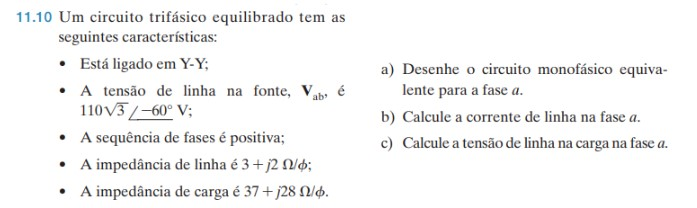
\includegraphics[scale=1.0]{P11.10.jpg}
\end{center}

\subsection*{(a)}

A tensão de linha da fonte trifásica é dada por  

\begin{equation}\label{eq:11.10.1}
    V_{ab} = V_a - V_b
\end{equation}

Como a sequências das fases é positiva, temos que a fase $a$ está adiantada em relação a fase $b$ de $120^{\circ}$.
Além disso, sabemos que a tensão de linha se relaciona com a tensão de fase através de    

\begin{equation}\label{eq:11.10.2}
    V_{ab} = |V_{an}|\sqrt{3}\phase{\phi_{an} \pm 30^{\circ}}
\end{equation}

Como a sequência de fases é positiva, usamos o sinal positivo para a fase em \eqref{eq:11.10.2}. Dessa forma, comparando
com o valor de $V_{ab} = 110\sqrt{3}\phase{-60^{\circ}}$ fornecido no enunciado, temos 

\[ \phi_{an} + 30^{\circ} = -60^{\circ} \logo \phi_{an} = -90^{\circ} \]

\[ |V_{ab}| = |V_{an}|\sqrt{3} \logo |V_{an}| = 110 \un{V} \]

Assim, a tensão de fase é dada por   

\[ V_{an} = 110\phase{-90^{\circ}} \un{V} \]

E o circuito monofásico equivalente da fase $a$ está exibido na Figura \ref*{fig:11.10.1}.

\begin{figure}[hb]
    \centering
    \caption{Circuito equivalente ao enunciado.}
      \centering
      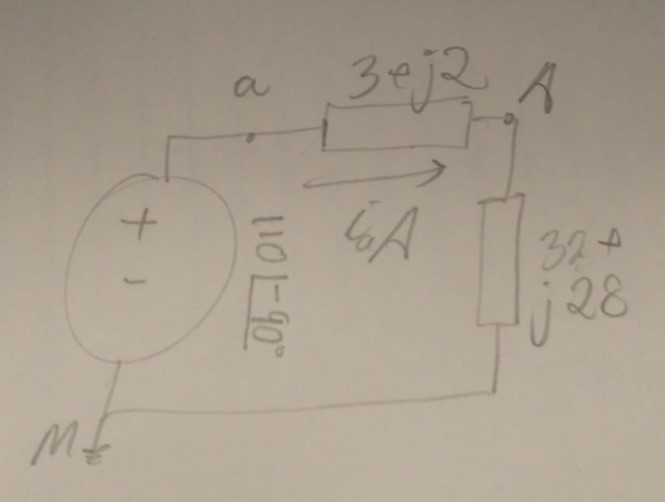
\includegraphics[scale=0.5]{P11.10-Item(a).jpg} \\
    \label{fig:11.10.1}
\end{figure}

\subsection*{(b)}

A corrente da fase $a$ é dada por   

\[ I_{aA} = \frac{V_{an}}{Z_{aA} + Z_L} \]

\[ I_{aA} = \frac{110\phase{-90^{\circ}}}{3 +j2 + 37 + j28} = \frac{110\phase{-90^{\circ}}}{40 + j30}  \]

\[ \boxed{I_{aA} = 2.2\phase{-126.87^{\circ}} \un{A}} \]

\subsection*{(c)}

A tensão na carga na fase $a$ é dada por   

\[ V_{AN} = Z_a \cdot I_{aA} = (37 + j28)(2.2\phase{-126.87^{\circ}}) \]

\[ V_{AN} = 102.08\phase{-89.75^{\circ}} \un{V}\]

A tensão de linha na carga, usando \eqref{eq:11.10.2},

\[ V_{AB} = 102.08\sqrt{3}\phase{-89.75 + 30^{\circ}} \un{V}\]

\[ \boxed{V_{AB} = 176.8\phase{59.75^{\circ}} \un{V}} \]



